\documentclass{article}

\usepackage[utf8]{inputenc}
\usepackage{amsmath}
\usepackage{amssymb}
\usepackage{anysize}
\usepackage{color}
\usepackage{xcolor}
\usepackage{graphicx}
\usepackage{float}

\usepackage{subfigure}

\usepackage{hyperref}


\definecolor{dkgreen}{rgb}{0, 0.6, 0}
\definecolor{gray}{rgb}{0.5, 0.5, 0.5}
\usepackage{listings}
\lstset{
	language=Matlab,                	% choose the language of the code
	keywords={break,case,catch,continue,else,elseif,end,for,function,
      global,if,otherwise,persistent,return,switch,try,while},
      keywordstyle=\color{blue},
      commentstyle=\color{red},
	basicstyle=\footnotesize,       % the size of the fonts that are used for the code
	numbers= left,                 	% where to put the line-numbers
	numberstyle=\footnotesize,      % the size of the fonts that are used for the line-numbers
	stepnumber=1,                   % the step between two line-numbers. If it is 1 each line will be numbered
	numbersep=5pt,                  % how far the line-numbers are from the code
	backgroundcolor=\color{white},  % choose the background color. You must add \usepackage{color}
	showspaces=false,               % show spaces adding particular underscores
	showstringspaces=false,         % underline spaces within strings
	showtabs=false,                 % show tabs within strings adding particular underscores
	frame=single,           		% adds a frame around the code
	tabsize=2,          			% sets default tabsize to 2 spaces
	captionpos=t,          			% sets the caption-position to bottom (t=top, b=bottom)
	breaklines=true,        		% sets automatic line breaking
	breakatwhitespace=false,    	% sets if automatic breaks should only happen at whitespace
	escapeinside={\%*}{*),  % if you want to add a comment within your code
	flexiblecolumns=true}         
}

\usepackage{caption}
\DeclareCaptionFont{white}{\color{white}}
\DeclareCaptionFormat{listing}{\colorbox{gray}{\parbox[c]{\textwidth}{#1#2#3}}}
\captionsetup[lstlisting]{format=listing,labelfont=white,textfont=white}

\setlength\parindent{0pt}
\setlength{\parskip}{10pt}

\marginsize{3cm}{2cm}{2cm}{2cm}

\title{Autonomous Robotics\\
		RRT Algorithm\\
		Lab 2 Report}
\author{Emre Ozan Alkan\\
		\{emreozanalkan@gmail.com\}\\
		MSCV-5}
\date{\today}

\begin{document}
\maketitle


\section{Introduction}

	Path planning also known as motion planning is an important task for autonomous robotics. It's aim is to find shortest or at least optimal path between start and goal positions. It is hard and highly demanded task today. In this lab, we implemented RRT (Rapidly-Exploring Random Trees) to solve simple path planning problem in Matlab.
	
	\subsection{Environment}
	In this lab, we had two 2D environment. In these environments; obstacles and empty spaces are marked as 1 and 0  respectively. We had to find optimal path between given start position and the goal position.
	
\begin{figure}[H]
\centering
\subfigure[683x803 Map Environment]{
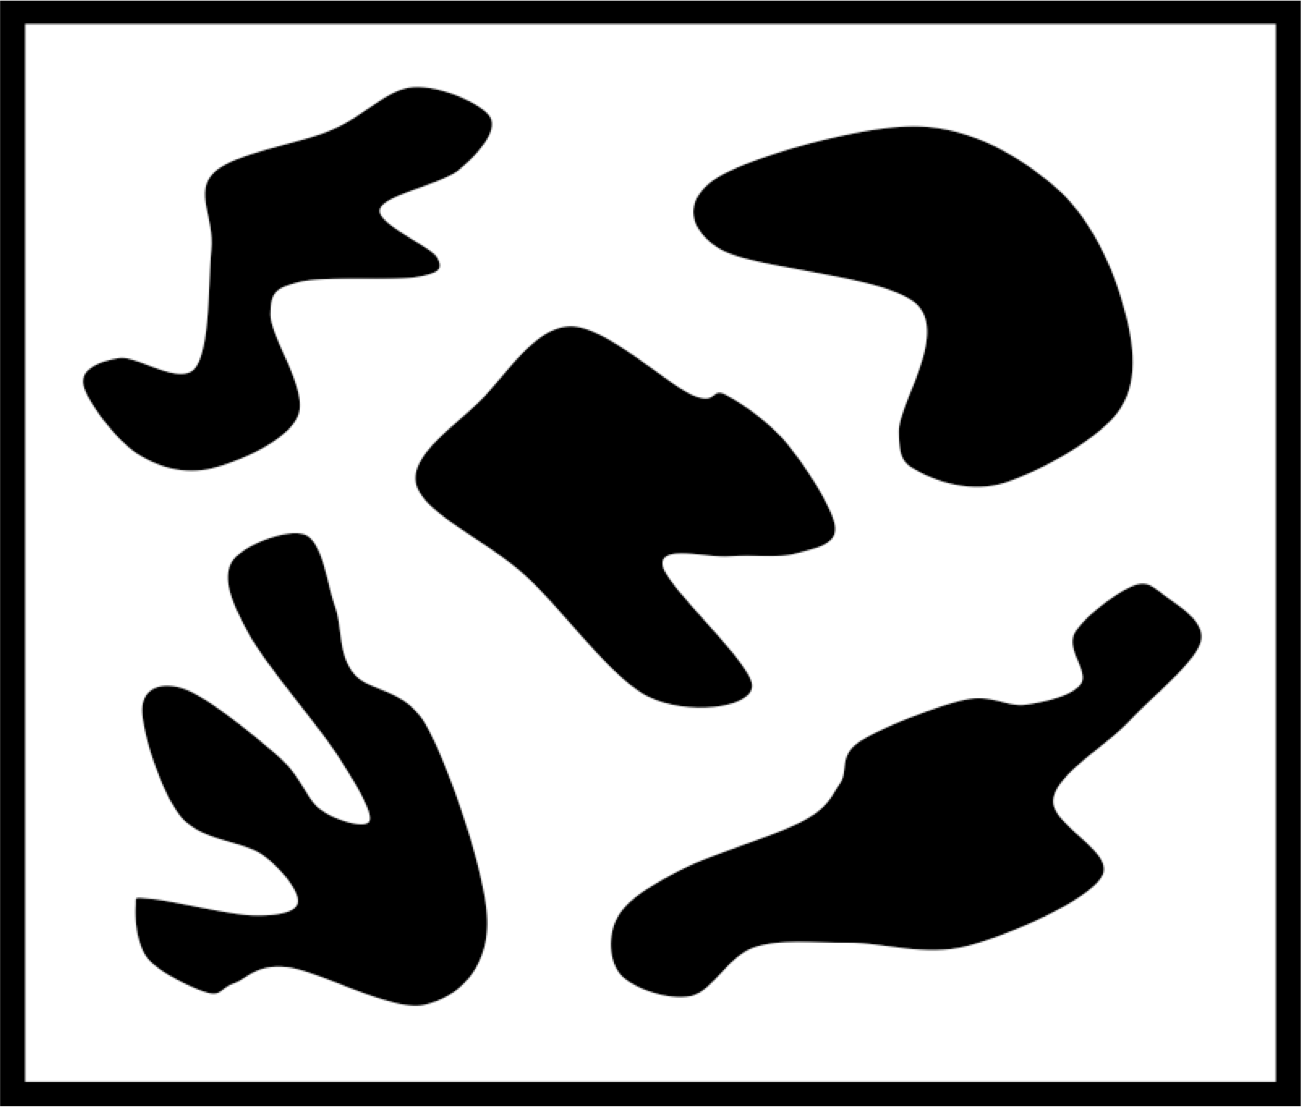
\includegraphics[width=.480\textwidth]{map.png}
}
\subfigure[687x802 Maze Environment]{
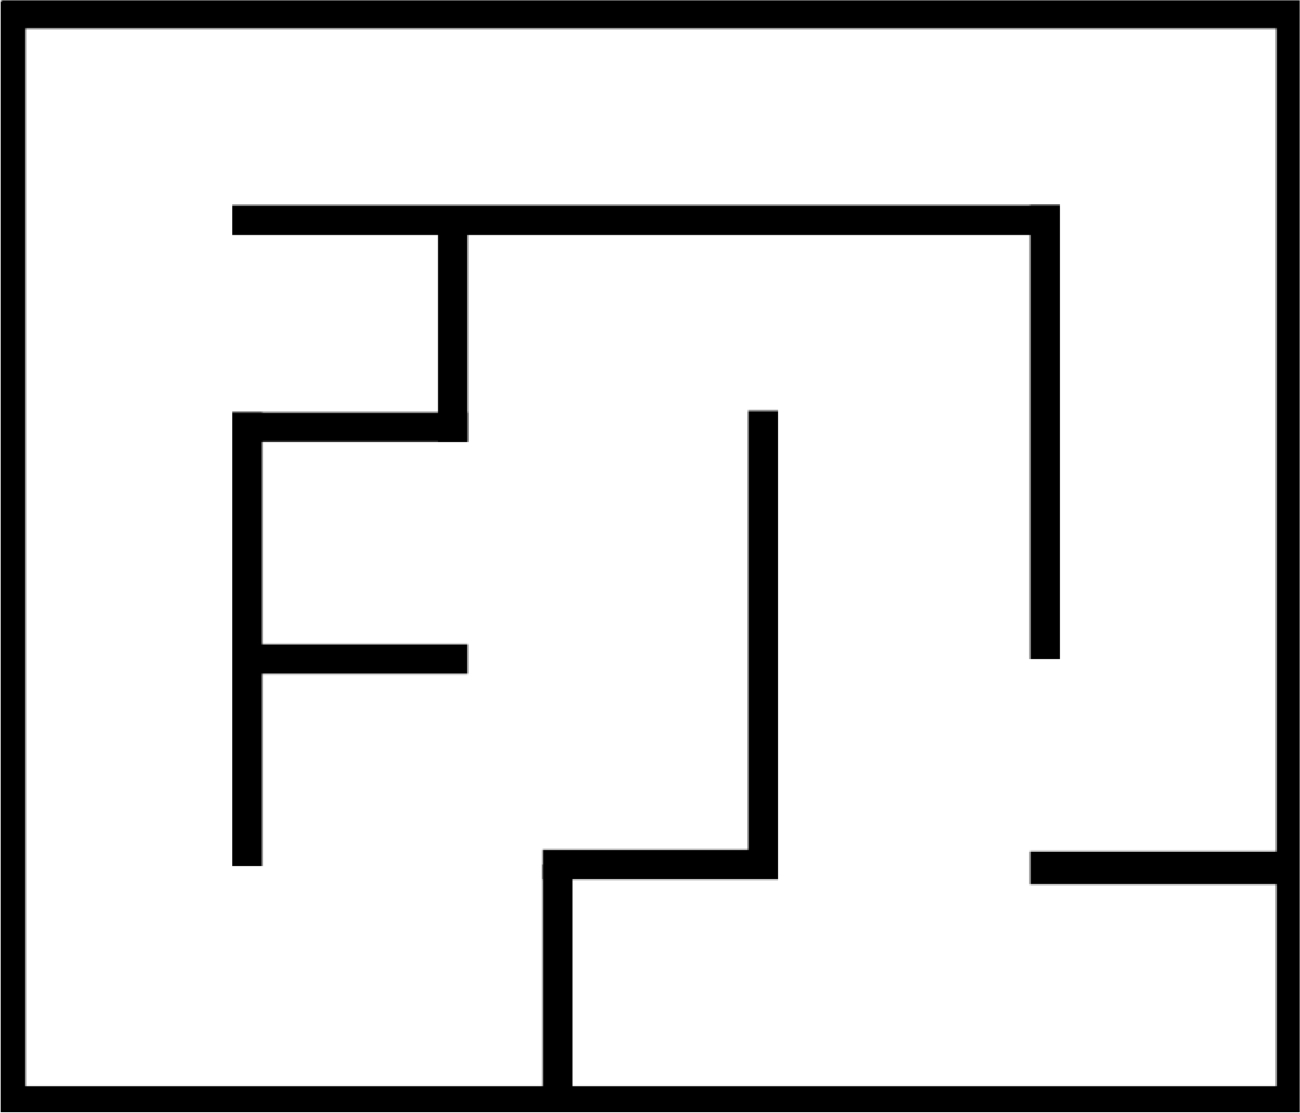
\includegraphics[width=.480\textwidth]{maze.png}
}
\caption{Sample Environments}
%\label{fig:whatever}
\end{figure}
	

	\subsection{RRT Algorithm}
	RRT algorithm is designed to search high dimensional spaces within configuration space by randomly building tree. It compose of creating randomly points or with some probabilty selecting goal, creating vertex and edge on that direction, and so on till it reaches the goal. \par
	So in this lab, we implemented RRT Algorithm that creating random points, searhing nearest vertices to that point, creating new point to that direction with given distance and checking if it and its edge belongs the free space, and so on till it reaches the goal.

\begin{figure}[H]
\begin{center}
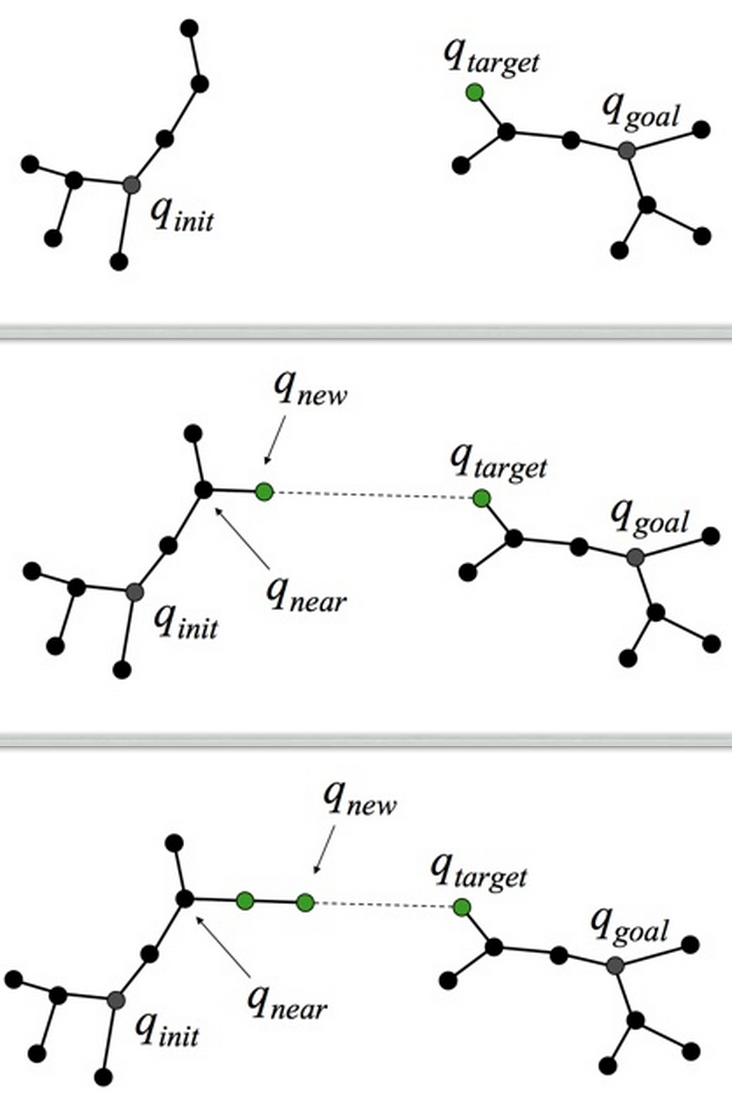
\includegraphics[scale=0.2]{RRTAlgorithm.png}
\caption{Graphical Demonstration of RRT Algorithm *[3]}
\end{center}
\end{figure}	

	\subsection{Path Smoothing}
	Since RRT algorithm creating random points, tend to build tree towards random points, mostly solution path is not optimal and very noisy. Hence, we need some kind of noise reduction method for our path. Therefore, we asked to implement smoothing method on path to get shorter and less noisy path. We used 'greedy approach' where each time we trying our connect our latest point with the start position and so on. 
	
\begin{figure}[H]
\begin{center}
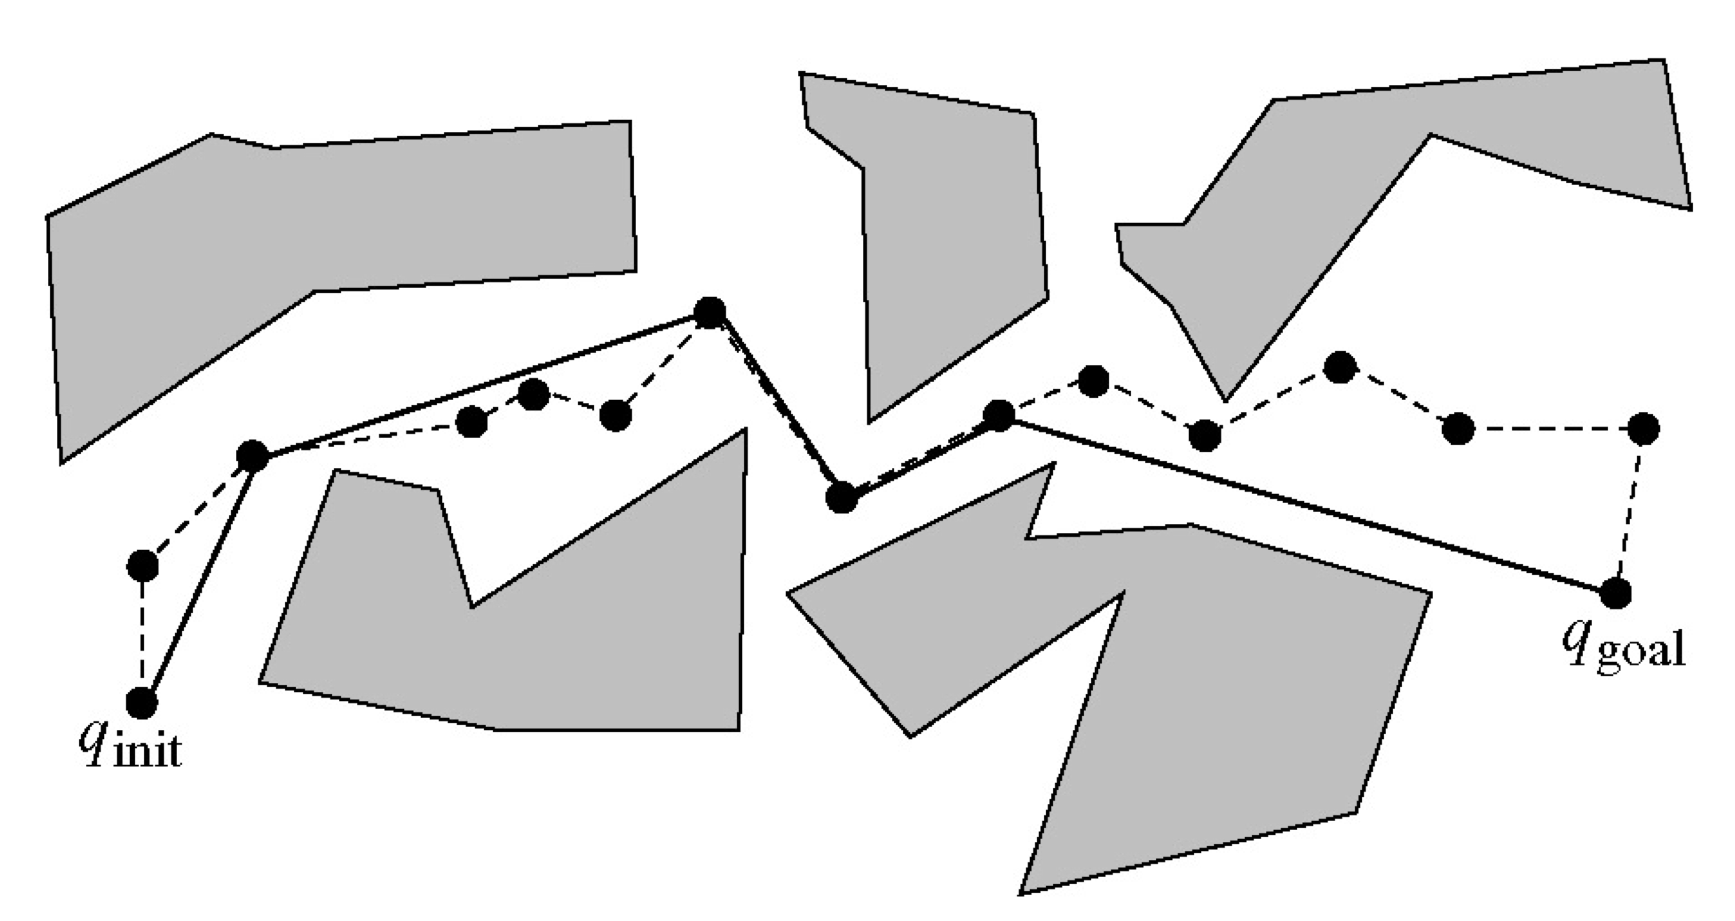
\includegraphics[scale=0.1]{rrtSmoothing.png}
\caption{Path Smoothing}
\end{center}
\end{figure}	
	
\section{Implementation}

Our RRT Algorithm implementation has two parts, RRT and smoothing for avoiding noises in RRT path. RRT find path but not shortest nor optimal. Smoothing method at least pruning the path, trying to connect points from goal to most reachable one, so path becomes more optimal.

	\subsection{Problems and Difficulties}
	In this lab I had difficulties on continuous coordinates and using these coordinates in right dimension of map. I had long debugging session to find a bug due to order of x and y coordinates where you already mentioned it in "important" title, but I forgot it.
	
		\subsubsection{Equation}
		One of the other difficulty was finding new point through randomly created point direction with given distance. In this part, I needed to read and search a lot. I decided to find vector and normalize it to find point with given distance. \par
		Lets $\mathbf q\_near = (x_1, y_1)$ and $\mathbf q\_rand = (x_0, y_0).$
		
		So $\mathbf v = q\_rand - q\_near $. We normalize this to $\mathbf u = \frac{\mathbf v}{||\mathbf v||}$ to get unit vector to use to find points with given distance.
		
		Then finding point with distance $d$ becomes easy:
		$qNew (x_3, y_3) =  q\_near + d \mathbf * u $
		
		After using the approach*[2] below, things became more clear.
		
		\subsubsection{Edge Free Space}
		Checking if edge belongs to free space was also challenging. Thanks to the approach above, and using 10 intermediate points as suggested, I was able to achieve it. This time, instead of checking with given distance, I divided my total distance between two points to number of intermediate point count, say delta\_q, and each iteration  I added delta\_q to get new coordinate and checked it if it belongs to free space.
	
	\subsection{Functions}
	Here is the the brief preview to functions I implemented to solve problem.
	
		\subsection{RRT}
		My RRT implementation consist of 6 main functions; 'rrt' - main function for algorithm, 'findQNear' - finding nearest vertices to created random point, 'findQNew' - finds point towards created random point with given delta distance, 'isEdgeQNearQNewBelongsFreeSpace' - checking if edge between q\_near and q\_new is belongs to free space, 'isQGoalOnQNearQNewEdge' - checking of goal is on the edge between q\_near and q\_new, 'fillSolutionPath' - creates solution path from given edges and vertices. \par
		
		Here are short preview to my rrt.m file with functions:

	\begin{lstlisting}[label=rrt-m, caption=rrt.m]
	
function [vertices, edges, path] = rrt(map, q_start, q_goal, k, delta_q, p)
tic;

clc;

if nargin < 3
    error('First 3 parameter is required: 2D map matrix, start and goal coordinates.');
elseif nargin < 4
    k = 10000;
    delta_q = 50;
    p = 0.3;
elseif nargin < 5
    delta_q = 50;
    p = 0.3;
elseif nargin < 6
    p = 0.3;
end

checkParameters(map, q_start, q_goal, k, delta_q, p);

% map: <683x803> means: height: 683, width: 803
[mapHeight, mapWidth] = size(map); % columns as the x axis and the rows as the y axis.

q_start = int32(q_start); % q_start = [80, 70] means: q_start(1): y, q_start(2): x
q_goal = int32(q_goal); % q_goal = [707, 615] means: q_goal(1): y, q_goal(2): x 
vertices = q_start; % Initialize the vertices variable with q_start

edges = int32.empty(0, 2); % Initialize the edges variable as empty

q_rand = int32.empty(0, 2);

q_near = int32.empty(0, 2);

q_new = int32.empty(0, 2);

for ii = 1 : k % For k samples repeat
    
    if rand() < p % With p probability use q_rand = q_goal
        q_rand = q_goal;
    else % Otherwise generate q_rand in the dimensions of the map.
        q_rand = int32([randi(mapWidth) randi(mapHeight)]); % columns as the x axis and the rows as the y axis.
    end
    
    [q_near, qNearIndex] = findQNear(q_rand, vertices); % Find q_near from q_rand in vertices
    
    q_new = findQNew(q_near, q_rand, delta_q); % Generate q_new at delta_q distance from q_near in the direction to q_rand
    
    if q_new(1) < 1 || q_new(2) < 1 || q_new(1) > mapWidth || q_new(2) > mapHeight
        continue;
    end
    
    if map(q_new(2), q_new(1)) == 0 % If q_new belongs to free space
        
        % If the edge between q_near and q_new belongs to free space
        if isEdgeQNearQNewBelongsFreeSpace(map, q_near, q_new)
            
            % Add q_new in vertices 
            vertices = [vertices; q_new];
            % Add [index(q_new) index(q_near)] in edges
            [qNewIndex, ~] = size(vertices);
            edges = [edges; [int32(qNewIndex), int32(qNearIndex)]];
            
            % If q_new == q_goal or q_goal is on the edge
            if isequal(q_new, q_goal) || isQGoalOnQNearQNewEdge(q_near, q_new, q_goal)
                
                if ~isequal(q_new, q_goal) % if goal is not q_new but its on edge
                    % goal is on the last edge, remove last vertex and add it as goal
                    vertices = vertices(1 : (end - 1), :);
                    vertices = [vertices; q_goal];
                end
                
                % Fill path and stop break RRT function
                path = fillSolutionPath(edges, vertices);
                
                % rrtDraw(map, q_start, q_goal, vertices, edges, path);
                
                toc;
                
                return;
            end
        end
    end
end

    path = int32.empty(0, 2);
    % rrtDraw(map, q_start, q_goal, vertices, edges, path);
    toc;
    
    error('RRT: solution not found :(');
end

function checkParameters(map, q_start, q_goal, k, delta_q, p)
...
end

% Find q_near from q_rand in vertices.
function [q_near, qNearIndex] = findQNear(q_rand, vertices)
...
end

% Generate q_new at delta_q distance from q_near in the direction to q_rand
function [q_new] = findQNew(q_near, q_rand, delta_q)
...
end

% If the edge between q_near and q_new belongs to free space
function [isBelongsFreeSpace] = isEdgeQNearQNewBelongsFreeSpace(map, q_near, q_new)
...
end

% q_near <--> q_goal <--> q_new
function [isQGoalOnEdge] = isQGoalOnQNearQNewEdge(q_near, q_new, q_goal)
...
end

% Fill path and stop break RRT function
function [path] = fillSolutionPath(edges, vertices)
...
end

% Plots the RRT result
function rrtDraw(map, q_start, q_goal, vertices, edges, path)
...
end


	\end{lstlisting}
		
		\subsection{Path Smoothing}
				My RRT Path Smoothing implementation consist of 2 main functions; 'smooth' - main function for smoothing path, 'isEdgeBelongsFreeSpace' - incrementally checking if edge between two point is belongs to free space with given delta distance.\par
		
		Here are short preview to my smooth.m file with functions:
		
	\begin{lstlisting}[label=smooth-m, caption=smooth.m]
	
function [path_smooth] = smooth(map, path, vertices, delta)

path_smooth = path(1); % initing with goal
currentIndex = 1; % path array iterator
currentSmoothIndex = numel(path); % path reverse array iterator

while currentIndex < numel(path)
    
    while currentIndex < currentSmoothIndex
        
        if isEdgeBelongsFreeSpace(map, vertices(path(currentSmoothIndex), :), vertices(path(currentIndex), :), delta)
            path_smooth = [path_smooth, path(currentSmoothIndex)];
            currentIndex = currentSmoothIndex;
            break;
        else
            currentSmoothIndex = currentSmoothIndex - 1;
        end
        
    end
    
    currentSmoothIndex = numel(path);
    
end

% rrtSmoothDraw(map, path_smooth, vertices);

end

function [isBelongsFreeSpace] = isEdgeBelongsFreeSpace(map, startPoint, endPoint, delta)
...
end

function rrtSmoothDraw(map, path_smooth, vertices)
...
end

	\end{lstlisting}

\section{Results}
	Here is the results I obtained with RRT algorithm, and after path smoothing. Parameters k, delta\_q, p and delta for smoothing is used as 10000, 50, 0.3 and 5 respectively.

	\subsection{RRT}
	
\begin{figure}[H]
\begin{center}
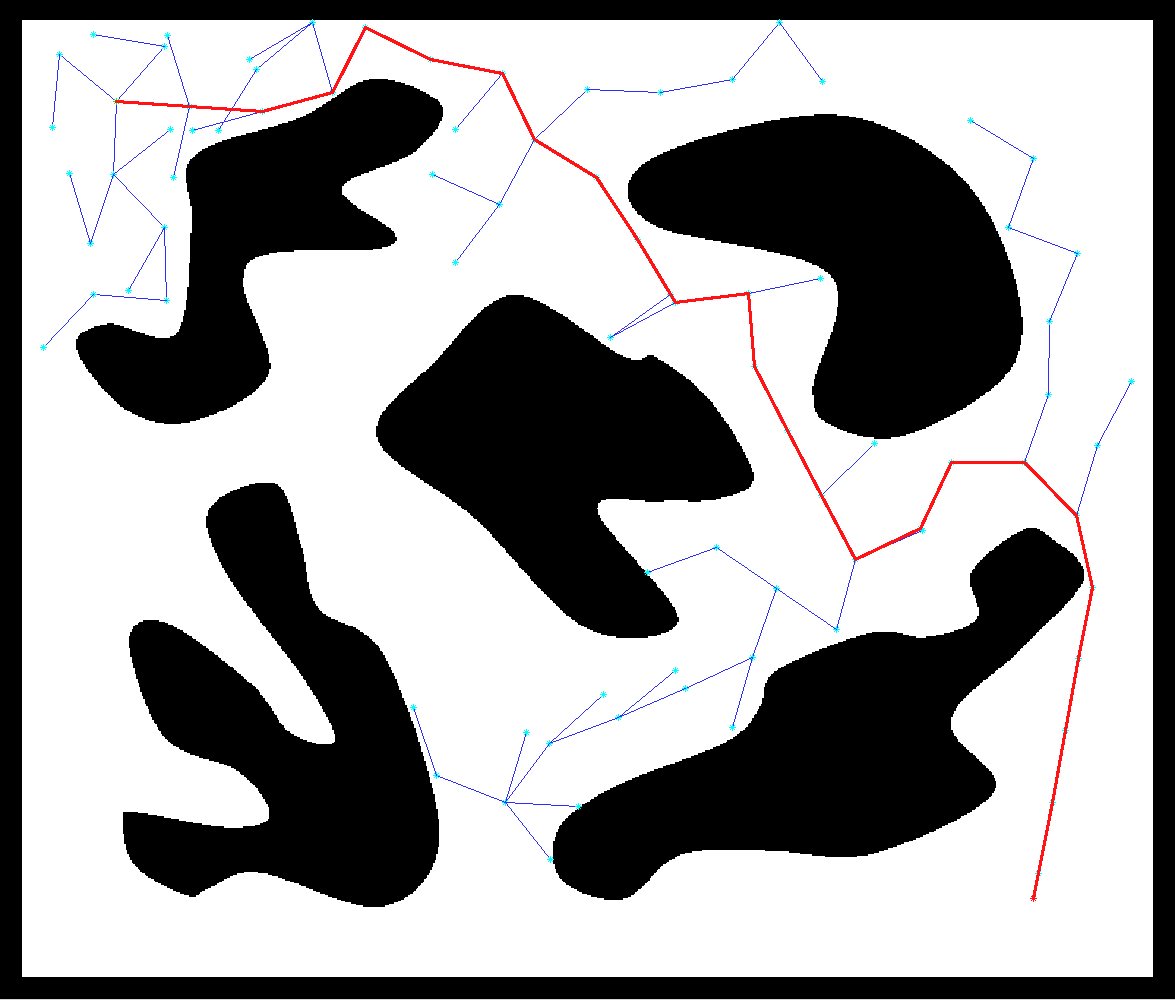
\includegraphics[scale=0.2]{rrtMap.png}
\caption{RRT Algorithm on Map}
\end{center}
\end{figure}	

\begin{figure}[H]
\begin{center}
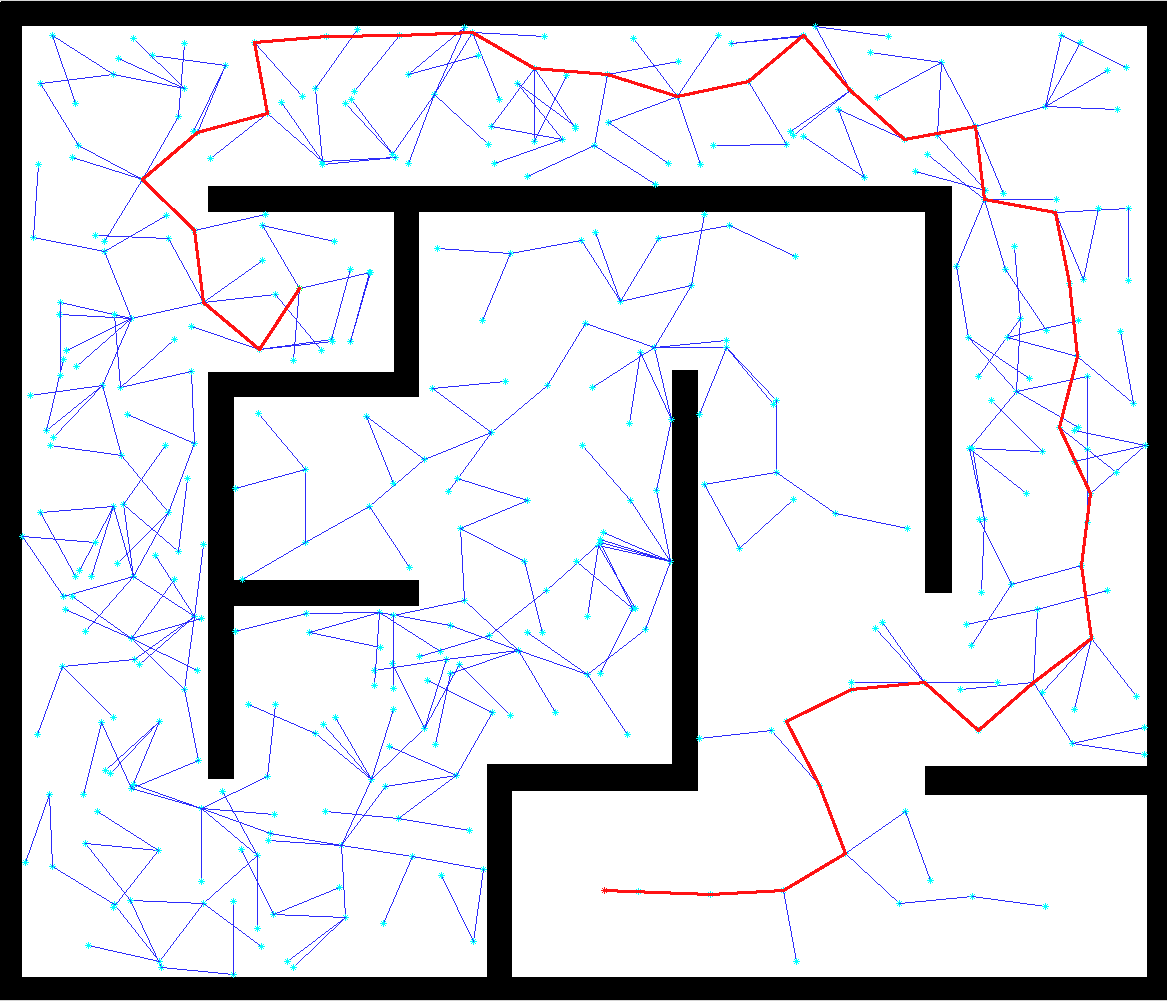
\includegraphics[scale=0.2]{rrtMaze.png}
\caption{RRT Algorithm on Maze}
\end{center}
\end{figure}	
	
	
	\subsection{Smoothing Path}
	
\begin{figure}[H]
\begin{center}
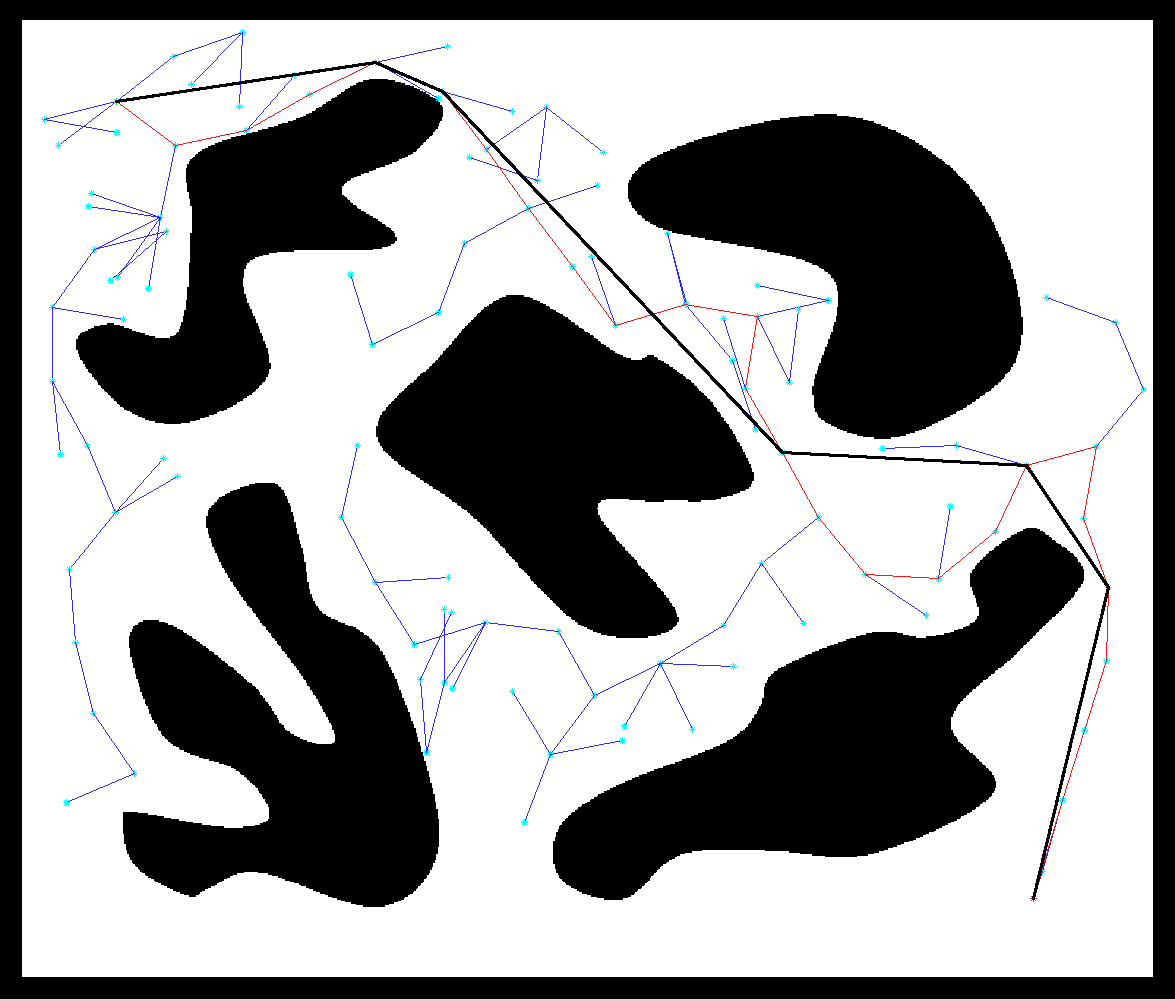
\includegraphics[scale=0.2]{smoothMap.png}
\caption{RRT with Smooth Path on Map}
\end{center}
\end{figure}	

\begin{figure}[H]
\begin{center}
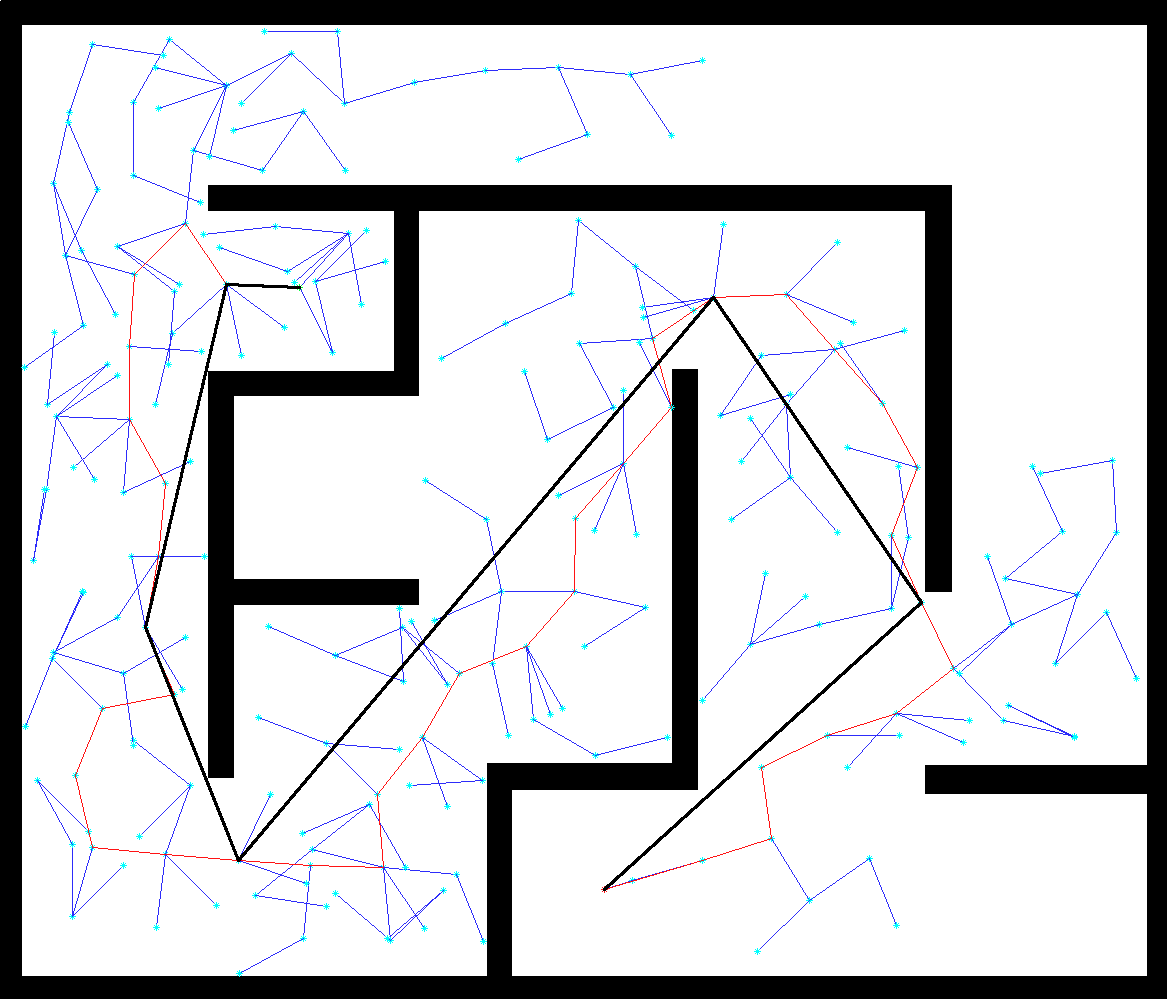
\includegraphics[scale=0.2]{smoothMaze.png}
\caption{RRT with Smooth Path on Maze}
\end{center}
\end{figure}	
	
\section{References}
\begin{enumerate}
	\item \href{url}{http://math.stackexchange.com/questions/175896/finding-a-point-along-a-line-a-certain-distance-away-from-another-point}
	\item \href{url}{http://stackoverflow.com/questions/1061276/how-to-normalize-a-vector-in-matlab-efficiently-any-related-built-in-function}
	\item \href{url}{http://kovan.ceng.metu.edu.tr/~asil/old/\_1./hw4.html}
	\item \href{url}{http://en.wikipedia.org/wiki/Rapidly\_exploring\_random\_tree}
\end{enumerate}


\end{document}